\section{Peer-to-Peer-Technologie}
\label{subsec:peer_to_peer_technologie}
% #TODO: Funktion des Kademlia Protokolls nennen und erklären (vielleicht in Grundlagen)
% Im Kademlia-Protokoll sind vier Funktionen definiert, die für die Suche nach
% Knoten und Werten verwendet werden. Diese Funktionen sind \texttt{FIND\_NODE},
% \texttt{FIND\_VALUE}, \texttt{PING} und \texttt{STORE}. Die Funktionen
% \texttt{FIND\_NODE} und \texttt{FIND\_VALUE} werden verwendet, um nach Knoten
% oder Werten zu suchen. Die Funktion \texttt{PING} wird verwendet, um die
% Erreichbarkeit eines Knotens zu überprüfen. Die Funktion \texttt{STORE} wird
% verwendet, um einen Wert in einem Knoten zu speichern.

Peer-to-Peer-Technologien können in zwei Kategorien unterteilt werden: Peer-to-Peer-Anwendungen und Peer-to-Peer-Infrastrukturen. Die Kategorie der Peer-to-Peer-Anwen-\\dungen umfasst den Dienst der Inhaltsverteilung, bei dem die Teilnehmer Inhalte wie Musik, Videos oder andere Dateien direkt untereinander austauschen \Parencite[730-731]{Khatibi_StructuredUnstructuredP2P}. 

Daher werden viele Peer-to-Peer schnell mit Filesharing in Verbindung bringen, da diese Technologie in der Vergangenheit vor allem dafür genutzt wurde. Das bekannteste Beispiel ist das Filesharing-Netzwerk \textit{Napster}, das 1999 von Shawn \enquote{Napster} Fanning entwickelt wurde. \textit{Napster} war das erste weit verbreitete Filesharing-Netzwerk, das auf Peer-to-Peer-Technologie basierte. Es ermöglichte den Austausch von Musikdateien zwischen den Teilnehmern. Die Musikdateien wurden dabei auf den Computern der Teilnehmer gespeichert und konnten von anderen Teilnehmern heruntergeladen werden. Da diese Art des Datenaustauschs oftmals illegal war, wurde Napster 2001 aufgrund von Urheberrechtsverletzungen abgeschaltet \parencite[S. 55-57]{Mahlmann_P2PNetzwerke}.

Die Peer-to-Peer-Infrastruktur umfasst die Peer-to-Peer-Netzwerke, die für die Kommunikation zwischen den Teilnehmern verwendet werden \parencite[S. 730-731]{Khatibi_StructuredUnstructuredP2P}. Diese Arbeit konzentriert sich auf die Peer-to-Peer-Infrastruktur, die die Kommunikation zwischen den Teilnehmern ermöglichen soll.

Im Instant-Messaging-Bereich repräsentiert das Peer-to-Peer-Modell eine dezentrale Struktur, die dabei hilft, die Kommunikation zwischen den Teilnehmern zu ermöglichen. Im Gegensatz zum Client-Server-Ansatz, bei dem ein zentraler Server die Kommunikation zwischen den Teilnehmern steuert, ermöglicht das Peer-to-Peer-Netzwerk direkte Kommunikation zwischen den Teilnehmern. Beide Modelle bringen Vor- und Nachteile mit sich. Während das Client-Server-Modell eine zentrale Instanz erfordert, um die Kommunikation zu verwalten, ist das Peer-to-Peer-Netzwerk dezentralisiert und benötigt keine solche Instanz. Die Implementierung und Wartung eines Client-Server-Modells gestalten sich einfacher im Vergleich zu einem komplexeren und aufwendigeren Peer-to-Peer-Netzwerk. Das Client-Server-Modell ist weniger flexibel, da es von einer zentralen Instanz abhängt, während das Peer-to-Peer-Netzwerk aufgrund des Fehlens dieser Instanz flexibler ist. Skalierbarkeit ist ebenfalls ein Unterschied: Das Client-Server-Modell ist durch die Kapazität des Servers begrenzt, während das Peer-to-Peer-Netzwerk auf die Kapazität der Teilnehmer zurückgreift, was seine Skalierbarkeit verbessert. In Bezug auf Sicherheit ist das Client-Server-Modell weniger robust, da es auf eine zentrale Instanz angewiesen ist, während das Peer-to-Peer-Netzwerk, das ohne solche Abhängigkeit auskommt, als sicherer gilt \parencite[S. 6-8]{Mahlmann_P2PNetzwerke}.


\subsection{Typen von Peer-to-Peer-Netzwerken}

Nicht jedes Peer-to-Peer-Netzwerk ist gleich. Es gibt verschiedene Typen von Peer-to-Peer-Netzwerken, die sich in ihrer Struktur und Funktionsweise unterscheiden. Abbildung \ref{p2p_typen} zeigt die zwei Haupttypen von Peer-to-Peer-Netzwerken: unstrukturierte und strukturierte Netzwerke \parencite[S. 362-363]{Luntovskyy_ModRechnernetze}.

\begin{center}
    \captionsetup{type=figure}
    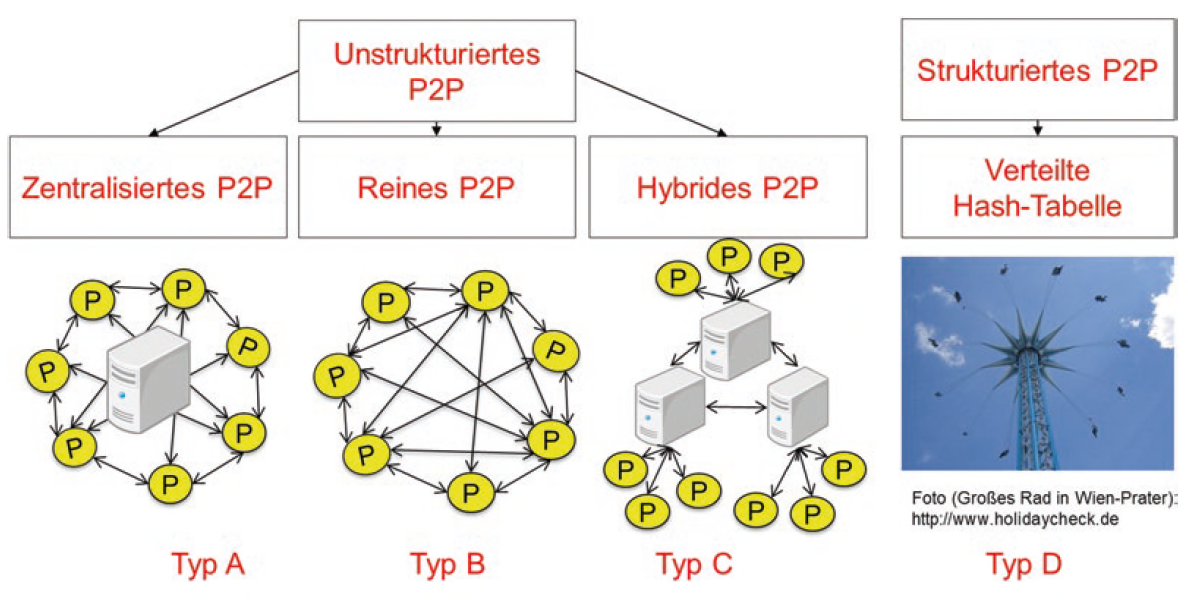
\includegraphics[width=1\linewidth]{images/peer_to_peer_typen.png}
    \captionof{figure}{Typen von Peer-to-Peer-Netzwerken \parencite{Luntovskyy_ModRechnernetze}}
    \label{p2p_typen}
\end{center}

\noindent Unstrukturierte und strukturierte Peer-to-Peer-Netzwerke sind unterschiedliche Ansätze zur Organisation von Knoten und Ressourcen in dezentralen Netzwerken.

Unstrukturierte Netzwerke sind charakterisiert durch ihre fehlende explizite Organisationsstruktur, was eine einfache Konnektivität ermöglicht. \textit{Typ A} in Abbildung \ref{p2p_typen} zeigt ein zentralisiertes Netzwerk, was bedeutet, dass alle Teilnehmer mit einem zentralen Server verbunden sind. Als Beispiel für diese Form des Peer-to-Peer dient \textit{Napster}. Bei \textit{Napster} gab es mehrere Server, die die Dateien der Teilnehmer indizierten. Die Teilnehmer konnten Dateien von anderen Teilnehmern herunterladen, indem sie eine Anfrage an einen der Server stellten, der dann die IP-Adresse des Teilnehmers zurückgab, der die Datei zur Verfügung stellte \parencite[S. 171]{Saroiu_MeasuringAndAnalyzingNapsterAndGnutellaHosts}. Diese Form ermöglicht eine schnelle und effiziente Suche nach Ressourcen, da die Ressourcen zentral verwaltet werden, aber die Abhängigkeit von einem zentralen Server macht das Netzwerk nicht skalierbar und anfällig für Ausfälle \parencite[S. 732]{Khatibi_StructuredUnstructuredP2P}.
Bei \textit{Typ B} handelt es sich um ein reines Peer-to-Peer-Netzwerk, bei dem die Teilnehmer direkt miteinander verbunden sind und jeder sowohl als Client als auch als Server fungiert \parencite[S. 732]{Khatibi_StructuredUnstructuredP2P}. Ein Beispiel für diese Form des Peer-to-Peer ist \textit{Gnutella}. Bei \textit{Gnutella} gab es keine zentrale Instanz, die die Ressourcen der Teilnehmer indizierte. Die Suche nach Ressourcen oder Informationen erfolgt durch Broadcasts oder zufällige Weiterleitungen, was jedoch zu ineffizienten Suchprozessen führen kann, da keine klare Routing-Struktur vorhanden ist \parencite[S. 171]{Saroiu_MeasuringAndAnalyzingNapsterAndGnutellaHosts}. Beim dritten und letzten Typ der unstrukturierten Netzwerke handelt es sich um ein hybrides Peer-to-Peer-Netzwerk, das Elemente aus den beiden anderen Typen kombiniert. In einem hybriden Netzwerk gibt es besondere Knoten (engl. Nodes), die die Funktionen eines Servers, wie beispielsweise Indexierung der Ressourcen, für eine bestimmte Gruppe von Teilnehmern übernehmen. Diese Knoten werden als Superknoten (engl. Super Nodes) bezeichnet. Die Super Nodes selbst sind untereinander dezentralisiert miteinander verbunden. Ein Beispiel für diese Form des Peer-to-Peer ist \textit{Gnutella2} \parencite[S. 732]{Khatibi_StructuredUnstructuredP2P}. 

Strukturierte Peer-to-Peer-Netzwerke hingegen weisen klare Regeln und Algorithmen zur Organisation der Knoten auf. Diese Netzwerke verfügen über eine explizite Organisationsstruktur, sei es eine Ringstruktur, k-bucket basierte Systeme oder andere, die es ermöglichen, effizientes Routing und eine optimierte Ressourcenverwaltung zu erreichen. Durch diese klar definierte Struktur sind strukturierte Netzwerke oft stabiler und bieten eine effizientere Ressourcenlokalisierung im Vergleich zu ihren unstrukturierten Gegenstücken. Allerdings kann diese Stabilität auf Kosten von Flexibilität und Anpassungsfähigkeit gehen, da Änderungen in der Netzwerktopologie oder hohe Dynamik der Knoten schwerer zu handhaben sind \textcolor{red}{[QUELLE]}.



\subsection{Problemstellung und mögliche Lösungen}

Peer-to-Peer-Netzwerke sind nicht ohne Probleme. Die dezentrale Struktur der Netzwerke bringt einige Herausforderungen mit sich, die es zu bewältigen gilt. Eines der Probleme stellen die \textit{Network Address Translators} (kurz: NATs) dar. NATs sind dafür zuständig, private IP-Adressen in öffentliche IP-Adressen umzuwandeln und umgekehrt. Sie werden in Routern oder Gateways eingesetzt und dienen dazu, den Zugang von Geräten im lokalen Netzwerk (die private IP-Adressen verwenden) zum Internet zu ermöglichen, indem sie den Datenverkehr zwischen dem lokalen Netzwerk und dem externen Netzwerk, wie dem Internet, verwalten. Peer-to-Peer Verbindungen stoßen bei Network Address Translators oft auf Probleme, was daran liegt, dass NATs normalerweise nicht erlauben, dass externe Geräte direkt mit internen kommunizieren. Zudem werden Ports dynamisch für ausgehenden Traffic zugewiesen, was das Weiterleiten eingehender Verbindungen erschwert. Symmetrische NATs verschärfen dieses Problem, da sie für ausgehende Verbindungen eine eindeutige Kombination von IP-Adresse und Port verwenden, die sich bei jeder neuen Verbindung ändert \Parencite[S. 1-9]{rfc2663_NAT_Terminology}.

Dies ist ein Problem, da die Teilnehmer nicht direkt miteinander kommunizieren können, wenn sie sich hinter einem NAT befinden. Um dieses Problem zu lösen, gibt es verschiedene Lösungsansätze. Einer davon ist das \textit{Relaying}. Beim Relaying wird ein Server als Vermittler zwischen den Teilnehmern verwendet. Die Teilnehmer verbinden sich mit dem Server und leiten ihren Datenverkehr über diesen Server weiter. 
Ein weiterer Ansatz ist die \textit{Connection Reversal}. Bei der Connection Reversal wird ein \textit{Rendezvous-Server} verwendet, um eine Verbindung zwischen den Teilnehmern herzustellen. Der Teilnehmer hinter dem NAT verbindet sich mit dem Rendezvous-Server und teilt diesem seine öffentliche IP-Adresse und Port mit. Der andere Teilnehmer verbindet sich ebenfalls mit dem Rendezvous-Server und erhält die IP-Adresse und Port des  Teilnehmers hinter dem NAT. Bei dieser Technik darf sich nur einer der Teilnehmer hinter einem NAT befinden.
\textit{Hole Punching} beschreibt einen weiteren Lösungsansatz. Zwei Geräte, die eine direkte Verbindung miteinander aufbauen möchten, initiieren gleichzeitig eine Verbindung zu einem Server, der sich außerhalb des NATs befindet. Der Server sammelt die IP-Adressen und Ports der beiden Geräte und leitet diese an die jeweils andere Partei weiter. Die beiden Geräte versuchen dann, eine Verbindung zueinander herzustellen, indem sie gleichzeitig Datenpakete an die IP-Adresse und den Port des anderen Geräts senden. Dabei wird versucht, das NAT dazu zu bringen, die Verbindung zu öffnen, indem es die ankommenden Pakete als Antwort auf die ausgehenden Pakete erkennt. Wenn dies gelingt, wird ein temporäres Loch im NAT geöffnet, das es den Geräten ermöglicht, direkt miteinander zu kommunizieren. Diese Technik erfordert eine präzise Koordination und die Fähigkeit der beiden Geräte zur gleichen Zeit Datenpakete zu senden und zu empfangen. Zudem ist es nicht immer möglich, ein temporäres Loch im NAT zu öffnen, da es von der Implementierung des NATs abhängt. Eine Abwandlung vom Hole Punching ist die \textit{Port Number Prediction}. Hierbei wird versucht, die Portnummer vorherzusagen, die das NAT für die Verbindung verwenden wird.Durch Beobachtung und Analyse vorheriger Verbindungen wird versucht Muster oder Trends in der Art und Weise zu erkennen, wie Portnummern zugewiesen werden. Dies könnte auf bestimmte Algorithmen oder Verhaltensweisen des Systems hinweisen, woraus dann die Portnummer vorhergesagt werden kann. Diese Technik ist jedoch nicht immer zuverlässig, da es rein auf Annahmen basiert und das Risiko besteht, dass sich das Portzuweisungsmuster jederzeit ändert \Parencite[S. 7-21]{rfc5128_P2P_NATs}.


Um die Problematik von Peer-to-Peer-Netzwerken zu lösen, können verschiedene Protokolle zum Einsatz kommen. Eines dieser Protokolle ist STUN (Session Traversal Utilities for NAT). STUN ist ein Netzwerkprotokoll, das es Geräten, die sich hinter einem NAT befinden, ermöglicht, ihre öffentliche IP-Adresse und Port zu ermitteln. Es bietet an sich keine Möglichkeit für eine Umgehung des NATs, sondern ist dafür gedacht, als eines von mehreren Werkzeugen verwendet zu werden, um ein NAT zu umgehen. Mittels STUN lässt sich nur ermitteln, ob sich ein Gerät hinter einem NAT befindet und welche IP-Adresse und Port es verwendet \parencite[S. 4]{rfc8489_STUN}.

TURN (Traversal Using Relays around NAT) ist ein weiteres Netzwerkprotokoll, das im Zusammenhang mit NATs verwendet wird. Aus der Spezifikation ist zu entnehmen, dass TURN ein Protokoll ist, das es Geräten, die sich hinter einem NAT befinden, ermöglicht, eine Verbindung zu einem anderen Gerät herzustellen, indem es einen Server als Vermittler verwendet. TURN ist ein Protokoll, das auf STUN aufbaut. Es bietet die gleichen Funktionalitäten wie STUN, aber zusätzlich die Möglichkeit, den Datenverkehr über einen Server zu leiten, um eine Verbindung zwischen zwei Geräten herzustellen. Das funktioniert auch, wenn sich beide Geräte hinter einem NAT befinden \parencite[S. 7]{rfc8656_TURN}.

ICE (Interactive Connectivity Establishment) ist ein Framework, das mehrere Techniken kombiniert, um eine Verbindung zwischen zwei Endpunkten herzustellen, die sich hinter NATs befinden. Es verwendet STUN und TURN, um die öffentliche IP-Adresse und Port eines Geräts zu ermitteln und den Datenverkehr über einen Server zu leiten \Parencite[S. 6]{rfc8445_ICE}.


\subsection{Overlay-Netzwerke(drin lassen?)}

Peer-to-Peer-Netzwerke können als Overlay-Netzwerk betrachtet werden. Ein Overlay-Netzwerk ist ein virtuelles Netzwerk, das über ein physisches Netzwerk gelegt wird. Es besteht aus einer Reihe von Knoten, die über eine logische Verbindung miteinander verbunden sind. Die Verbindungen zwischen den Knoten werden durch Routing-Algorithmen verwaltet. Die Knoten können sich über das physische Netzwerk befinden, aber auch über das Internet verteilt sein \parencite{Lua_P2POverlayNetworksPaper}. 

Beispiele für Routing-Algorithmen sind \textit{Kademlia}, \textit{Chord} und \textit{Pastry}. All diese Algorithmen verwenden sogenannte \textit{Distributed Hash Tables}, um die Knoten zu verwalten. Eine \textit{Distributed Hash Table} (kurz: DHT) ist eine verteilte Datenstruktur, die es ermöglicht, Daten in einem Netzwerk zu speichern und zu verwalten. Sie besteht aus einer Reihe von Knoten, die miteinander verbunden sind und die Daten speichern. Die Knoten sind über das Netzwerk verteilt und die Daten werden wiederum auf die Knoten verteilt und in Form von Schlüssel-Wert-Paaren gespeichert. Die Schlüssel werden dabei gehasht, um die Daten auf die Knoten zu verteilen. Die Knoten speichern nur die Daten, die sich in ihrem Verantwortungsbereich befinden. Wenn ein Knoten eine Anfrage für einen bestimmten Schlüssel erhält, leitet er die Anfrage an den Knoten weiter, der für diesen Schlüssel verantwortlich ist. Dieser Knoten antwortet dann mit dem entsprechenden Wert. Die DHTs sind selbstorganisierend, was bedeutet, dass sie sich selbst verwalten und anpassen können, wenn sich die Netzwerktopologie ändert. Kademlia, Chord und Pastry sind Beispiele für die Implementierung von DHTs \parencite[S. 1-2]{Maymounkov_Kademlia} \parencite[S. 1-2]{Stoica_Chord} \parencite[S. 1-2]{Rowstron_Pastry}.

\subsection{Kademlia, Chord, Pastry}

\textit{Kademlia} ist ein Peer-to-Peer-Protokoll, das für die Organisation von Knoten in einem Netzwerk verwendet wird. Es ist ein strukturiertes Peer-to-Peer-Netzwerk, das auf einer K-Bucket-Struktur basiert. Die K-Buckets enthalten eine Liste von Knoten für verschiedene Schlüsselbereiche basierend auf ihrer Nähe, die durch XOR-Distanzen der IDs berechnet wird. Die Verbindungen zwischen den Knoten sind asymmetrisch, und jeder Knoten speichert Informationen über andere Knoten in seinen K-Buckets. Bei der Suche nach einem bestimmten Schlüssel erfolgt das Routing durch die XOR-Entfernung, wodurch die nächsten Knoten für diesen Schlüssel gefunden werden. Dieses Verfahren ermöglicht eine logarithmische Anzahl von Schritten für die Suche und bietet eine robuste Struktur, die gut mit dynamischen Netzwerkänderungen umgehen kann \parencite[S. 1-2]{Maymounkov_Kademlia}.

\textit{Chord} ist ein weiteres Peer-to-Peer-Protokoll, das für die Organisation von Knoten in einem Netzwerk verwendet wird. Es ist ebenfalls ein strukturiertes Peer-to-Peer-Netzwerk, basiert allerdings auf einer Ringstruktur. Die Knoten sind in einem Ring angeordnet und jeder Knoten ist für einen bestimmten Schlüsselbereich verantwortlich. Die Verbindungen zwischen den Knoten sind durch ihren Platz im Ring definiert, wobei jeder Knoten eine Verbindung zu seinem nächsten Nachbarn im Uhrzeigersinn hat. Bei der Suche nach einem bestimmten Schlüssel durchläuft eine Anfrage einen logarithmischen Pfad im Ring, wobei die Knoten auf dem Weg begrenzte Informationen über andere Knoten behalten, um Anfragen weiterzuleiten. Dieses Modell ist recht einfach und effizient für viele Anwendungsfälle, aber es könnte anfällig sein für Engpässe oder längere Suchzeiten, insbesondere wenn das Netzwerk dynamisch ist und sich die Konfiguration häufig ändert \parencite[S. 1-2]{Stoica_Chord}.

Auch \textit{Pastry} findet Anwendung als Peer-to-Peer-Protokoll zur Organisation von Knoten in einem Netzwerk. Es ist ein strukturiertes Peer-to-Peer-Netzwerk, das auf einer Baumstruktur basiert 




% #TODO: Overlay Netzwerk erklären? Kademlia ist ein Overlay Netzwerk
\begin{itemize}
    \item Was gibt es so für P2P-Protokolle/Algorithmen Chord, Kademlia, Pastry, Tapestry, CAN + DHTs + Churnrate
    \item Kademlia vs. Angriffe
    \item Angriffe gegen ICE gucken und erklären
\end{itemize}

%Firewalls können ebenfalls ein Problem darstellen, da sie den Datenverkehr zwischen dem lokalen Netzwerk und dem externen Netzwerk überwachen und filtern. Sie können den Datenverkehr blockieren, wenn sie verdächtige Aktivitäten erkennen. Dies kann dazu führen, dass die Teilnehmer nicht miteinander kommunizieren können.
